% Options for packages loaded elsewhere
\PassOptionsToPackage{unicode}{hyperref}
\PassOptionsToPackage{hyphens}{url}
%
\documentclass[
]{article}
\usepackage{amsmath,amssymb}
\usepackage{iftex}
\ifPDFTeX
  \usepackage[T1]{fontenc}
  \usepackage[utf8]{inputenc}
  \usepackage{textcomp} % provide euro and other symbols
\else % if luatex or xetex
  \usepackage{unicode-math} % this also loads fontspec
  \defaultfontfeatures{Scale=MatchLowercase}
  \defaultfontfeatures[\rmfamily]{Ligatures=TeX,Scale=1}
\fi
\usepackage{lmodern}
\ifPDFTeX\else
  % xetex/luatex font selection
\fi
% Use upquote if available, for straight quotes in verbatim environments
\IfFileExists{upquote.sty}{\usepackage{upquote}}{}
\IfFileExists{microtype.sty}{% use microtype if available
  \usepackage[]{microtype}
  \UseMicrotypeSet[protrusion]{basicmath} % disable protrusion for tt fonts
}{}
\makeatletter
\@ifundefined{KOMAClassName}{% if non-KOMA class
  \IfFileExists{parskip.sty}{%
    \usepackage{parskip}
  }{% else
    \setlength{\parindent}{0pt}
    \setlength{\parskip}{6pt plus 2pt minus 1pt}}
}{% if KOMA class
  \KOMAoptions{parskip=half}}
\makeatother
\usepackage{xcolor}
\usepackage[margin=1in]{geometry}
\usepackage{color}
\usepackage{fancyvrb}
\newcommand{\VerbBar}{|}
\newcommand{\VERB}{\Verb[commandchars=\\\{\}]}
\DefineVerbatimEnvironment{Highlighting}{Verbatim}{commandchars=\\\{\}}
% Add ',fontsize=\small' for more characters per line
\usepackage{framed}
\definecolor{shadecolor}{RGB}{248,248,248}
\newenvironment{Shaded}{\begin{snugshade}}{\end{snugshade}}
\newcommand{\AlertTok}[1]{\textcolor[rgb]{0.94,0.16,0.16}{#1}}
\newcommand{\AnnotationTok}[1]{\textcolor[rgb]{0.56,0.35,0.01}{\textbf{\textit{#1}}}}
\newcommand{\AttributeTok}[1]{\textcolor[rgb]{0.13,0.29,0.53}{#1}}
\newcommand{\BaseNTok}[1]{\textcolor[rgb]{0.00,0.00,0.81}{#1}}
\newcommand{\BuiltInTok}[1]{#1}
\newcommand{\CharTok}[1]{\textcolor[rgb]{0.31,0.60,0.02}{#1}}
\newcommand{\CommentTok}[1]{\textcolor[rgb]{0.56,0.35,0.01}{\textit{#1}}}
\newcommand{\CommentVarTok}[1]{\textcolor[rgb]{0.56,0.35,0.01}{\textbf{\textit{#1}}}}
\newcommand{\ConstantTok}[1]{\textcolor[rgb]{0.56,0.35,0.01}{#1}}
\newcommand{\ControlFlowTok}[1]{\textcolor[rgb]{0.13,0.29,0.53}{\textbf{#1}}}
\newcommand{\DataTypeTok}[1]{\textcolor[rgb]{0.13,0.29,0.53}{#1}}
\newcommand{\DecValTok}[1]{\textcolor[rgb]{0.00,0.00,0.81}{#1}}
\newcommand{\DocumentationTok}[1]{\textcolor[rgb]{0.56,0.35,0.01}{\textbf{\textit{#1}}}}
\newcommand{\ErrorTok}[1]{\textcolor[rgb]{0.64,0.00,0.00}{\textbf{#1}}}
\newcommand{\ExtensionTok}[1]{#1}
\newcommand{\FloatTok}[1]{\textcolor[rgb]{0.00,0.00,0.81}{#1}}
\newcommand{\FunctionTok}[1]{\textcolor[rgb]{0.13,0.29,0.53}{\textbf{#1}}}
\newcommand{\ImportTok}[1]{#1}
\newcommand{\InformationTok}[1]{\textcolor[rgb]{0.56,0.35,0.01}{\textbf{\textit{#1}}}}
\newcommand{\KeywordTok}[1]{\textcolor[rgb]{0.13,0.29,0.53}{\textbf{#1}}}
\newcommand{\NormalTok}[1]{#1}
\newcommand{\OperatorTok}[1]{\textcolor[rgb]{0.81,0.36,0.00}{\textbf{#1}}}
\newcommand{\OtherTok}[1]{\textcolor[rgb]{0.56,0.35,0.01}{#1}}
\newcommand{\PreprocessorTok}[1]{\textcolor[rgb]{0.56,0.35,0.01}{\textit{#1}}}
\newcommand{\RegionMarkerTok}[1]{#1}
\newcommand{\SpecialCharTok}[1]{\textcolor[rgb]{0.81,0.36,0.00}{\textbf{#1}}}
\newcommand{\SpecialStringTok}[1]{\textcolor[rgb]{0.31,0.60,0.02}{#1}}
\newcommand{\StringTok}[1]{\textcolor[rgb]{0.31,0.60,0.02}{#1}}
\newcommand{\VariableTok}[1]{\textcolor[rgb]{0.00,0.00,0.00}{#1}}
\newcommand{\VerbatimStringTok}[1]{\textcolor[rgb]{0.31,0.60,0.02}{#1}}
\newcommand{\WarningTok}[1]{\textcolor[rgb]{0.56,0.35,0.01}{\textbf{\textit{#1}}}}
\usepackage{graphicx}
\makeatletter
\def\maxwidth{\ifdim\Gin@nat@width>\linewidth\linewidth\else\Gin@nat@width\fi}
\def\maxheight{\ifdim\Gin@nat@height>\textheight\textheight\else\Gin@nat@height\fi}
\makeatother
% Scale images if necessary, so that they will not overflow the page
% margins by default, and it is still possible to overwrite the defaults
% using explicit options in \includegraphics[width, height, ...]{}
\setkeys{Gin}{width=\maxwidth,height=\maxheight,keepaspectratio}
% Set default figure placement to htbp
\makeatletter
\def\fps@figure{htbp}
\makeatother
\setlength{\emergencystretch}{3em} % prevent overfull lines
\providecommand{\tightlist}{%
  \setlength{\itemsep}{0pt}\setlength{\parskip}{0pt}}
\setcounter{secnumdepth}{-\maxdimen} % remove section numbering
\ifLuaTeX
  \usepackage{selnolig}  % disable illegal ligatures
\fi
\usepackage{bookmark}
\IfFileExists{xurl.sty}{\usepackage{xurl}}{} % add URL line breaks if available
\urlstyle{same}
\hypersetup{
  pdftitle={DATA 405 Assignment 4},
  pdfauthor={Rin Meng 51940633},
  hidelinks,
  pdfcreator={LaTeX via pandoc}}

\title{DATA 405 Assignment 4}
\author{Rin Meng 51940633}
\date{}

\begin{document}
\maketitle

\section{Question 1}\label{question-1}

The binomial probability mass function (PMF) for the number successes
\(k\) (insect surviving) is given by

\[P(X=k) = \binom{n}{k} p^k (1-p)^{n-k}\]

where \(n\) is the number of trials (insect released), \(p\) is the
probability of success (insect surviving).

Applying the Maximum Likelihood Estimate (MLE) to the binomial PMF, we
have \[L(p) = \binom{100}{56} p^{56} (1-p){1-p}^{44}\] Now we minimize
the log-likelihood function \(l(p) = \log L(p)\) to find the MLE of
\(p\). \[l(p) = \log \binom{100}{56} + 56 \log p + 44 \log (1-p)\]
\[\frac{\partial l}{\partial p} = \frac{56}{p} - \frac{44}{1-p} = 0 \Leftrightarrow \frac{56}{p} = \frac{44}{1-p}\]
\[56 - 56p = 44p \Leftrightarrow 56 = 100p\] \[p = 0.56\] Therefore, the
maximum likelihood estimate for the probability that an insect survives
is \(p\) is 0.56.

Now we find the probability that more than 50 insects survive in a new
experiment.

\begin{Shaded}
\begin{Highlighting}[]
\FunctionTok{pbinom}\NormalTok{(}\DecValTok{50}\NormalTok{, }\DecValTok{100}\NormalTok{, }\FloatTok{0.56}\NormalTok{, }\AttributeTok{lower.tail =} \ConstantTok{FALSE}\NormalTok{)}
\end{Highlighting}
\end{Shaded}

\begin{verbatim}
## [1] 0.8659234
\end{verbatim}

Therefore, the probability that more than 50 insects survive in a new
experiment is 0.866.

\section{Question 2}\label{question-2}

\begin{Shaded}
\begin{Highlighting}[]
\NormalTok{DAX }\OtherTok{\textless{}{-}}\NormalTok{ EuStockMarkets[,}\DecValTok{1}\NormalTok{] }\CommentTok{\# extract the data}
\NormalTok{DAXlogreturn }\OtherTok{\textless{}{-}} \FunctionTok{diff}\NormalTok{(}\FunctionTok{log}\NormalTok{(DAX)) }\CommentTok{\# (a) calculate the log returns}
\NormalTok{drift }\OtherTok{\textless{}{-}} \FunctionTok{mean}\NormalTok{(DAXlogreturn) }\CommentTok{\# (b)}
\FunctionTok{acf}\NormalTok{(DAXlogreturn) }\CommentTok{\# (c) no substantial autocorrelations present}
\end{Highlighting}
\end{Shaded}

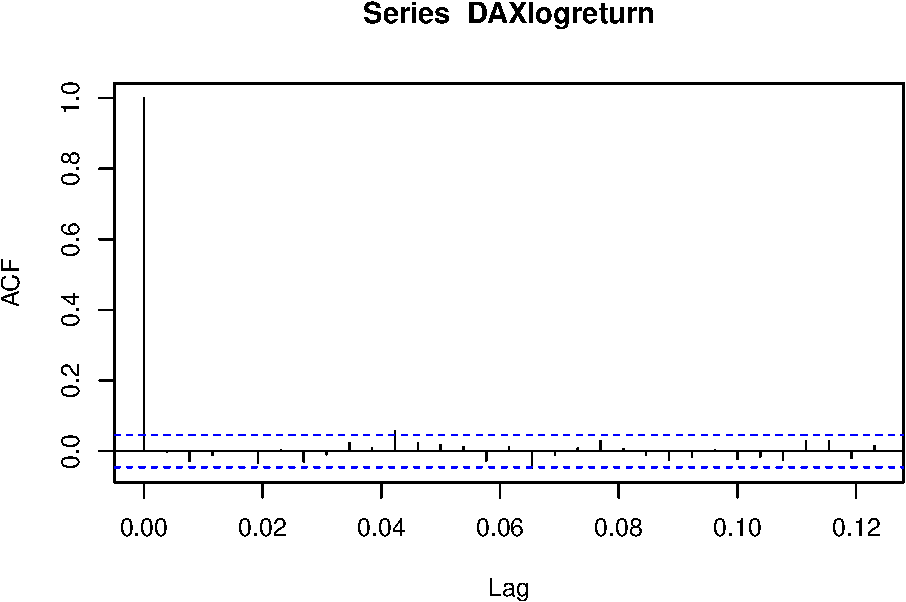
\includegraphics{a4_files/figure-latex/unnamed-chunk-2-1.pdf}

\begin{Shaded}
\begin{Highlighting}[]
\FunctionTok{acf}\NormalTok{(DAXlogreturn}\SpecialCharTok{\^{}}\DecValTok{2}\NormalTok{) }\CommentTok{\# (d) autocorrelations up to lag 2 present}
\end{Highlighting}
\end{Shaded}

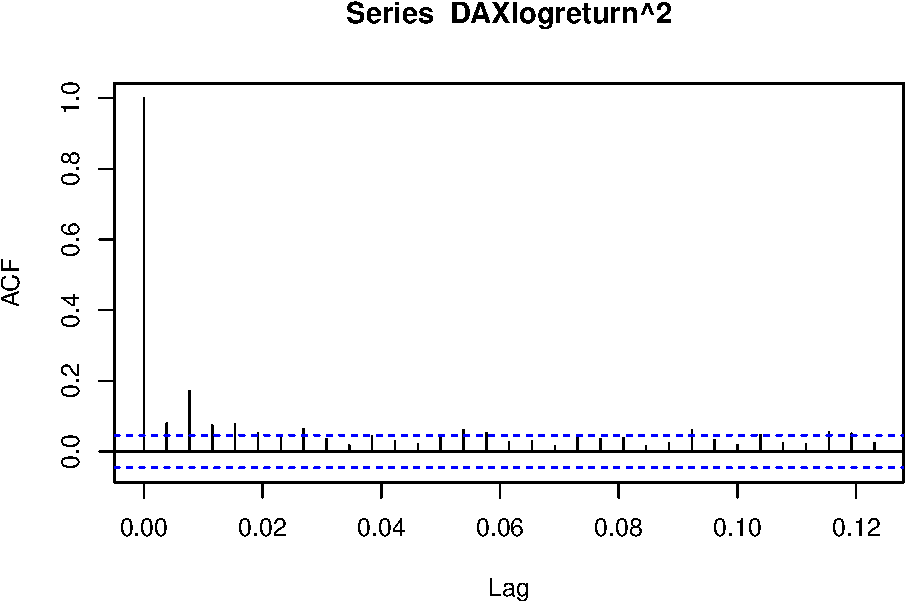
\includegraphics{a4_files/figure-latex/unnamed-chunk-2-2.pdf}

\begin{Shaded}
\begin{Highlighting}[]
\NormalTok{out }\OtherTok{\textless{}{-}} \FunctionTok{arima}\NormalTok{(DAXlogreturn}\SpecialCharTok{\^{}}\DecValTok{2}\NormalTok{, }\AttributeTok{order=}\FunctionTok{c}\NormalTok{(}\DecValTok{2}\NormalTok{, }\DecValTok{0}\NormalTok{, }\DecValTok{0}\NormalTok{)) }\CommentTok{\# (e)}
\NormalTok{phi }\OtherTok{\textless{}{-}}\NormalTok{ out}\SpecialCharTok{$}\NormalTok{coef[}\DecValTok{1}\SpecialCharTok{:}\DecValTok{2}\NormalTok{]; xbar }\OtherTok{\textless{}{-}}\NormalTok{ out}\SpecialCharTok{$}\NormalTok{coef[}\DecValTok{3}\NormalTok{]; s2 }\OtherTok{\textless{}{-}}\NormalTok{ out}\SpecialCharTok{$}\NormalTok{sigma2}
\NormalTok{n }\OtherTok{\textless{}{-}} \FunctionTok{length}\NormalTok{(DAX)}
\CommentTok{\# Simulate from this model \# (f)}
\NormalTok{y }\OtherTok{\textless{}{-}} \FunctionTok{numeric}\NormalTok{(n)}
\NormalTok{y[}\DecValTok{1}\SpecialCharTok{:}\DecValTok{2}\NormalTok{] }\OtherTok{\textless{}{-}} \FunctionTok{diff}\NormalTok{(}\FunctionTok{log}\NormalTok{(DAX))[}\DecValTok{1}\SpecialCharTok{:}\DecValTok{2}\NormalTok{] }\CommentTok{\# starting values for process}
\NormalTok{Z }\OtherTok{\textless{}{-}} \FunctionTok{rnorm}\NormalTok{(n) }\CommentTok{\# standard normals used in ARCH}
\ControlFlowTok{for}\NormalTok{ (i }\ControlFlowTok{in} \DecValTok{3}\SpecialCharTok{:}\NormalTok{n) \{}
\NormalTok{s }\OtherTok{\textless{}{-}} \FunctionTok{sqrt}\NormalTok{(xbar }\SpecialCharTok{+}\NormalTok{ phi[}\DecValTok{1}\NormalTok{]}\SpecialCharTok{*}\NormalTok{y[i}\DecValTok{{-}1}\NormalTok{]}\SpecialCharTok{\^{}}\DecValTok{2} \SpecialCharTok{+}\NormalTok{ phi[}\DecValTok{2}\NormalTok{]}\SpecialCharTok{*}\NormalTok{y[i}\DecValTok{{-}2}\NormalTok{]}\SpecialCharTok{\^{}}\DecValTok{2}\NormalTok{)}\SpecialCharTok{*}\NormalTok{Z[i]}
\NormalTok{y[i] }\OtherTok{\textless{}{-}}\NormalTok{ s}
\NormalTok{\}}
\CommentTok{\# y contains log returns, but an initial value is needed to}
\CommentTok{\# re{-}accumulate the prices, and the drift term must be added in:}
\NormalTok{y }\OtherTok{\textless{}{-}} \FunctionTok{c}\NormalTok{(}\FunctionTok{log}\NormalTok{(DAX[}\DecValTok{1}\NormalTok{]), y }\SpecialCharTok{+}\NormalTok{ drift)}
\NormalTok{DAXsim }\OtherTok{\textless{}{-}} \FunctionTok{exp}\NormalTok{(}\FunctionTok{cumsum}\NormalTok{(y)) }\CommentTok{\# simulated prices}
\FunctionTok{par}\NormalTok{(}\AttributeTok{mfrow=}\FunctionTok{c}\NormalTok{(}\DecValTok{1}\NormalTok{, }\DecValTok{2}\NormalTok{)) }\CommentTok{\# (g) compare trace plots of real and simulated data.}
\FunctionTok{ts.plot}\NormalTok{(DAX)}
\FunctionTok{ts.plot}\NormalTok{(DAXsim)}
\end{Highlighting}
\end{Shaded}

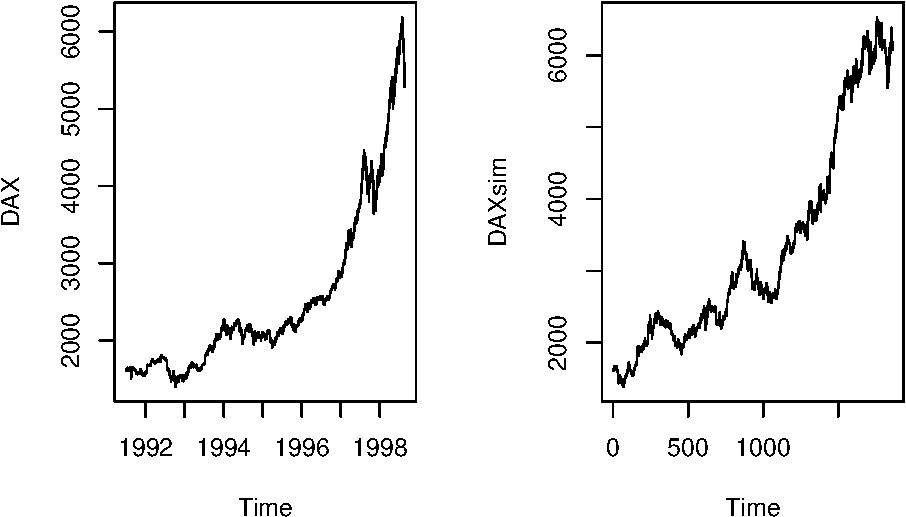
\includegraphics{a4_files/figure-latex/unnamed-chunk-2-3.pdf} (c) There
are no autocorrelations that are significant enough.

\begin{enumerate}
\def\labelenumi{(\alph{enumi})}
\setcounter{enumi}{3}
\tightlist
\item
  Yes there are autocorrelations up to lag 2 present. \# Question 3
\end{enumerate}

\begin{Shaded}
\begin{Highlighting}[]
\CommentTok{\# Load the CAC data (3rd column of EuStockMarkets)}
\NormalTok{CAC }\OtherTok{\textless{}{-}}\NormalTok{ EuStockMarkets[, }\DecValTok{3}\NormalTok{]}

\CommentTok{\# Step 1: Calculate the log returns for the CAC data}
\NormalTok{CAClogreturn }\OtherTok{\textless{}{-}} \FunctionTok{diff}\NormalTok{(}\FunctionTok{log}\NormalTok{(CAC))}

\CommentTok{\# Step 2: Check for autocorrelations in the squared log returns}
\FunctionTok{acf}\NormalTok{(CAClogreturn}\SpecialCharTok{\^{}}\DecValTok{2}\NormalTok{) }\CommentTok{\# This helps confirm the presence of ARCH effects}
\end{Highlighting}
\end{Shaded}

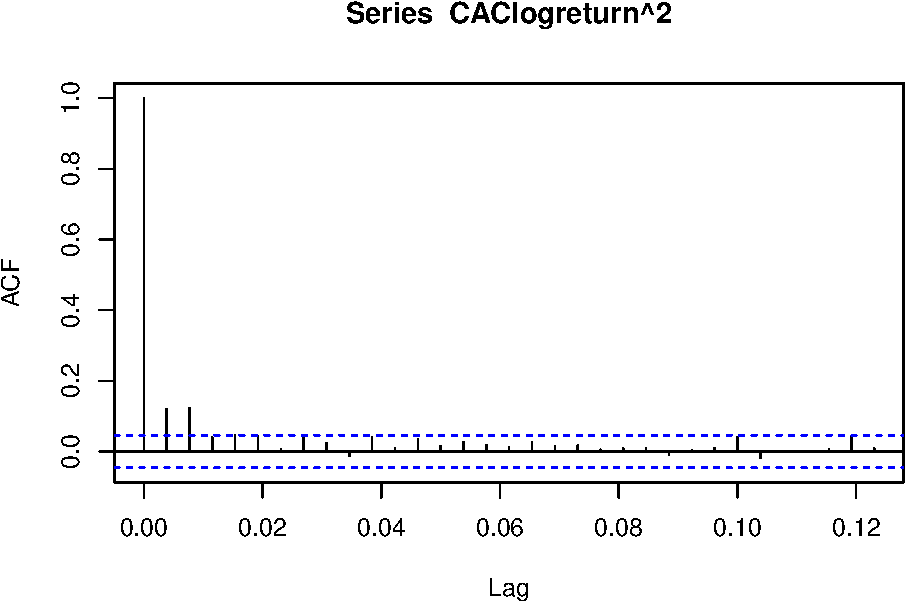
\includegraphics{a4_files/figure-latex/unnamed-chunk-3-1.pdf}

\begin{Shaded}
\begin{Highlighting}[]
\CommentTok{\# Step 3: Fit an ARCH(2) model to the squared log returns}
\NormalTok{out }\OtherTok{\textless{}{-}} \FunctionTok{arima}\NormalTok{(CAClogreturn}\SpecialCharTok{\^{}}\DecValTok{2}\NormalTok{, }\AttributeTok{order =} \FunctionTok{c}\NormalTok{(}\DecValTok{2}\NormalTok{, }\DecValTok{0}\NormalTok{, }\DecValTok{0}\NormalTok{))}
\NormalTok{phi }\OtherTok{\textless{}{-}}\NormalTok{ out}\SpecialCharTok{$}\NormalTok{coef[}\DecValTok{1}\SpecialCharTok{:}\DecValTok{2}\NormalTok{]   }\CommentTok{\# ARCH coefficients}
\NormalTok{xbar }\OtherTok{\textless{}{-}}\NormalTok{ out}\SpecialCharTok{$}\NormalTok{coef[}\DecValTok{3}\NormalTok{]    }\CommentTok{\# Intercept term}
\NormalTok{s2 }\OtherTok{\textless{}{-}}\NormalTok{ out}\SpecialCharTok{$}\NormalTok{sigma2       }\CommentTok{\# Residual variance}
\NormalTok{n }\OtherTok{\textless{}{-}} \FunctionTok{length}\NormalTok{(CAClogreturn)}

\CommentTok{\# Step 4: Simulate a new series with the same properties}
\NormalTok{y }\OtherTok{\textless{}{-}} \FunctionTok{numeric}\NormalTok{(n) }\CommentTok{\# Initialize the simulated log returns}
\NormalTok{y[}\DecValTok{1}\SpecialCharTok{:}\DecValTok{2}\NormalTok{] }\OtherTok{\textless{}{-}}\NormalTok{ CAClogreturn[}\DecValTok{1}\SpecialCharTok{:}\DecValTok{2}\NormalTok{] }\CommentTok{\# Use the first two log returns as starting values}
\NormalTok{Z }\OtherTok{\textless{}{-}} \FunctionTok{rnorm}\NormalTok{(n) }\CommentTok{\# Generate standard normal random variables for the ARCH model}

\ControlFlowTok{for}\NormalTok{ (i }\ControlFlowTok{in} \DecValTok{3}\SpecialCharTok{:}\NormalTok{n) \{}
\NormalTok{  s }\OtherTok{\textless{}{-}} \FunctionTok{sqrt}\NormalTok{(xbar }\SpecialCharTok{+}\NormalTok{ phi[}\DecValTok{1}\NormalTok{] }\SpecialCharTok{*}\NormalTok{ y[i}\DecValTok{{-}1}\NormalTok{]}\SpecialCharTok{\^{}}\DecValTok{2} \SpecialCharTok{+}\NormalTok{ phi[}\DecValTok{2}\NormalTok{] }\SpecialCharTok{*}\NormalTok{ y[i}\DecValTok{{-}2}\NormalTok{]}\SpecialCharTok{\^{}}\DecValTok{2}\NormalTok{) }\SpecialCharTok{*}\NormalTok{ Z[i]}
\NormalTok{  y[i] }\OtherTok{\textless{}{-}}\NormalTok{ s}
\NormalTok{\}}

\CommentTok{\# Add drift and re{-}accumulate prices to generate the simulated price series}
\NormalTok{drift }\OtherTok{\textless{}{-}} \FunctionTok{mean}\NormalTok{(CAClogreturn) }\CommentTok{\# Calculate the drift term}
\NormalTok{y }\OtherTok{\textless{}{-}} \FunctionTok{c}\NormalTok{(}\FunctionTok{log}\NormalTok{(CAC[}\DecValTok{1}\NormalTok{]), y }\SpecialCharTok{+}\NormalTok{ drift) }\CommentTok{\# Add drift and initial log price}
\NormalTok{CACsim }\OtherTok{\textless{}{-}} \FunctionTok{exp}\NormalTok{(}\FunctionTok{cumsum}\NormalTok{(y)) }\CommentTok{\# Convert log returns back to prices}

\CommentTok{\# Step 5: Plot the original and simulated data}
\FunctionTok{par}\NormalTok{(}\AttributeTok{mfrow =} \FunctionTok{c}\NormalTok{(}\DecValTok{1}\NormalTok{, }\DecValTok{2}\NormalTok{)) }\CommentTok{\# Arrange plots side by side}
\FunctionTok{ts.plot}\NormalTok{(CAC, }\AttributeTok{main =} \StringTok{"Original CAC Data"}\NormalTok{, }\AttributeTok{col =} \StringTok{"blue"}\NormalTok{)}
\FunctionTok{ts.plot}\NormalTok{(CACsim, }\AttributeTok{main =} \StringTok{"Simulated CAC Data"}\NormalTok{, }\AttributeTok{col =} \StringTok{"red"}\NormalTok{)}
\end{Highlighting}
\end{Shaded}

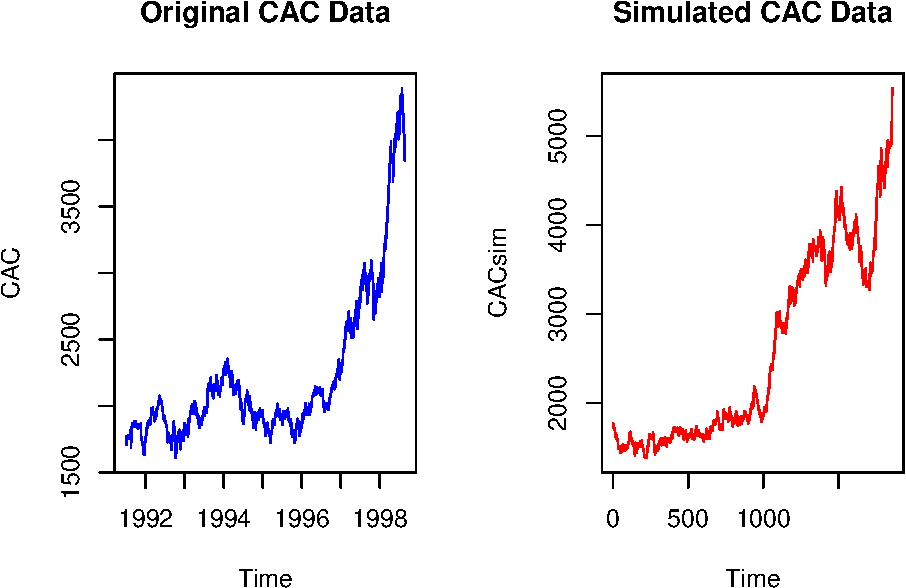
\includegraphics{a4_files/figure-latex/unnamed-chunk-3-2.pdf}

\section{Question 4}\label{question-4}

\begin{enumerate}
\def\labelenumi{(\alph{enumi})}
\tightlist
\item
  Finding the transition matrix, first we consider that the state space
  is \(S = \{0, 1, 2, 3\}\), where \(X_n\) is the number of containers
  in the yard at time \(n\).
\end{enumerate}

\begin{itemize}
\tightlist
\item
  Arrival Rule: A container arrives unless the yard is full, which is at
  state 3.
\item
  Removal Rule: Each container is independently removed with probability
  \(p = 0.8\)
\end{itemize}

At state 0, (\(X_n = 0\)):

\begin{itemize}
\item
  \(P(0 \rightarrow 1) = 0\) (no container arrives)
\item
  \(P(0 \rightarrow 0) = 1\) (no container is removed)
\end{itemize}

At state 1, (\(X_n = 1\)):

\begin{itemize}
\item
  \(P(1 \rightarrow 0) = 0\) (not possible since atleast a container
  arrives)
\item
  \(P(1 \rightarrow 1) = (1 - p) = 0.2\) (container is removed with
  probability 0.8)
\item
  \(P(1 \rightarrow 2) = p = 0.8\) (container arrives with probability
  0.8)
\item
  \(P(1 \rightarrow 3) = 0\) (we cannot reach 3 directly from state 1)
\end{itemize}

At state 2, (\(X_n = 2\)):

\begin{itemize}
\item
  \(P(0 \text{ containers removed}) = (1-p)^2 = 0.2^2 = 0.04\)
\item
  \(P(1 \text{ container removed}) = 2p(1-p) = 2 \times 0.8 \times 0.2 = 0.32\)
\item
  \(P(2 \text{ containers removed}) = p^2 = 0.8^2 = 0.64\)
\end{itemize}

Thus,

\begin{itemize}
\item
  \(P(2 \rightarrow 1) = P(1 \text{ containers removed}) = 0.32\)
\item
  \(P(2 \rightarrow 2) = P(0 \text{ containers removed}) = 0.04\)
\item
  \(P(2 \rightarrow 3) = P(2 \text{ containers removed}) = 0.64\)
\end{itemize}

At state 3, (\(X_n = 3\)):

\begin{itemize}
\item
  \(P(0 \text{ containers removed}) = (1-p)^3 = 0.2^3 = 0.008\)
\item
  \(P(1 \text{ container removed}) = 3p(1-p)^2 = 3 \times 0.8 \times 0.2^2 = 0.096\)
\item
  \(P(2 \text{ containers removed}) = 3p^2(1-p) = 3 \times 0.8^2 \times 0.2 = 384\)
\item
  \(P(3 \text{ containers removed}) = p^3 = 0.8^3 = 0.512\)
\end{itemize}

Thus,

\begin{itemize}
\item
  \(P(3 \rightarrow 0) = P(0 \text{ containers removed}) = 0.512\)
\item
  \(P(3 \rightarrow 1) = P(1 \text{ container removed}) = 0.384\)
\item
  \(P(3 \rightarrow 2) = P(2 \text{ containers removed}) = 0.096\)
\item
  \(P(3 \rightarrow 3) = P(3 \text{ containers removed}) = 0.096\)
\end{itemize}

Then, the transition matrix is given by

\[P = 
\begin{bmatrix} 
0 & 1 & 0 & 0 \\ 
0 & 0.2 & 0.8 & 0 \\ 
0 & 0.32 & 0.04 & 0.64 \\ 
0.512 & 0.384 & 0.096 & 0.008 
\end{bmatrix}\]

\begin{enumerate}
\def\labelenumi{(\alph{enumi})}
\setcounter{enumi}{1}
\tightlist
\item
  Probability of \(X_3 = 3\) given that \(X_1 = 2\) is given by
\end{enumerate}

\[P(X_3 = 3 | X_1 = 2) = P^2[2,3]\]

\begin{Shaded}
\begin{Highlighting}[]
\NormalTok{P }\OtherTok{\textless{}{-}} \FunctionTok{matrix}\NormalTok{(}
  \FunctionTok{c}\NormalTok{(}\DecValTok{0}\NormalTok{, }\DecValTok{1}\NormalTok{, }\DecValTok{0}\NormalTok{, }\DecValTok{0}\NormalTok{, }
    \DecValTok{0}\NormalTok{, }\FloatTok{0.2}\NormalTok{, }\FloatTok{0.8}\NormalTok{, }\DecValTok{0}\NormalTok{, }
    \DecValTok{0}\NormalTok{, }\FloatTok{0.32}\NormalTok{, }\FloatTok{0.04}\NormalTok{, }\FloatTok{0.64}\NormalTok{, }
    \FloatTok{0.512}\NormalTok{, }\FloatTok{0.384}\NormalTok{, }\FloatTok{0.096}\NormalTok{, }\FloatTok{0.008}\NormalTok{), }\AttributeTok{nrow =} \DecValTok{4}\NormalTok{, }\AttributeTok{byrow =} \ConstantTok{TRUE}\NormalTok{)}

\NormalTok{P2 }\OtherTok{\textless{}{-}}\NormalTok{ P }\SpecialCharTok{\%*\%}\NormalTok{ P}
\NormalTok{P2[}\DecValTok{3}\NormalTok{, }\DecValTok{4}\NormalTok{]}
\end{Highlighting}
\end{Shaded}

\begin{verbatim}
## [1] 0.03072
\end{verbatim}

Therefore, the probability of \(X_3 = 3\) given that \(X_1 = 2\) is
0.030.

\begin{enumerate}
\def\labelenumi{(\alph{enumi})}
\setcounter{enumi}{2}
\item
  A state space is defined as irreductible if every state can be reached
  from every other state, possibly over multiple steps Here, we see that
  it can eventually transition to the other states, via arrivals and
  removals. Thus, the state space is irreductible.
\item
  The limiting distribution \(\pi = (\pi_0, \pi_1, \pi_2, \pi_3)\)
  satisfies:
\end{enumerate}

\begin{itemize}
\item
  \(\pi = \pi P\)
\item
  \(\sum_{i=0}^{3} \pi_i = 1\)
\end{itemize}

Then we need to find that \[\pi_0 = 0.512\pi_3\]
\[\pi_1 = 0.384\pi_3 + 1\pi_0\] \[\pi_2 = 0.096\pi_3 + 0.8\pi_1\]
\[\pi_3 = 0.008\pi_3 + 0.64\pi_2\]

\end{document}
